\chapter{Summarized Algorithm}\label{secSummarizedApproach}

%A high-level overview of the algorithm is presented in figure \ref{figSummary}.
This chapter presents a summary of the defined algorithm. At first a short overview is provided followed by a description of the key aspects compared to a typical \gls{EvolutionaryAlgorithm}.

In general, the algorithm evolves a small subset of all possible \glspl{ModelToModelTransformation}, the \gls{Population}, through pattern based \glspl{Mutation}. It is guided by reference examples M$_a$ and M$_b^*$, which are input and expected output. 

By comparing the actual output M$_b$ with the expected M$_b^*$ created by a domain expert, the algorithm is able to rate the fitness of a \gls{ModelToModelTransformation}. Based on the fitness, the algorithm decides which existing \glspl{ModelToModelTransformation} are evolved using a Selection and Replacement Strategy. Such an evolution is the mutation of a \gls{ModelToModelTransformation} using a pattern-based \gls{Mutation}. Since there are many possible \glspl{Mutation}, the selection is performed by a Mutation Selection Strategy.

% \begin{figure}[!ht]
	% \centering
	% 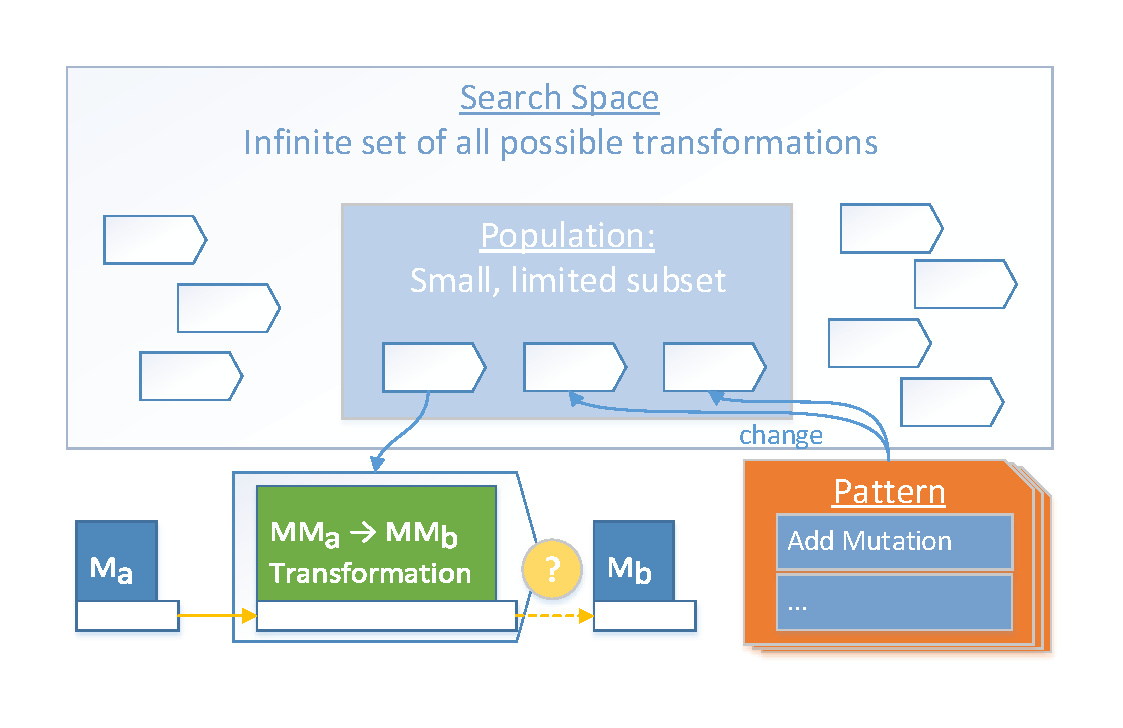
\includegraphics[scale=0.6, trim=0cm 1cm 0cm 1cm, clip=true]{Images/Summary.pdf} 
	% \caption{High-Level Algorithm Overview}
	% \label{figSummary}
% \end{figure}

Both \gls{ModelToModelTransformation} scenarios presented in chapter \ref{chapM2MScenarios} are usually solved by the implemented prototype in less than two hours. The resulting source code is maintainable in terms of readability and test-coverage, but the complex scenario contained solutions which lacked an easy comprehensibility.

Figure \ref{figFocusDistribution} presents an overview of the overall complexity distributed among the algorithm aspects. The classification of the typical distribution is not the result of an in depth analysis of the domain, but rather a selective observation. In general, this approach is not typical in the domain of \glspl{EvolutionaryAlgorithm}, which is outlined in the following.

\begin{figure}[!ht]
	\centering
	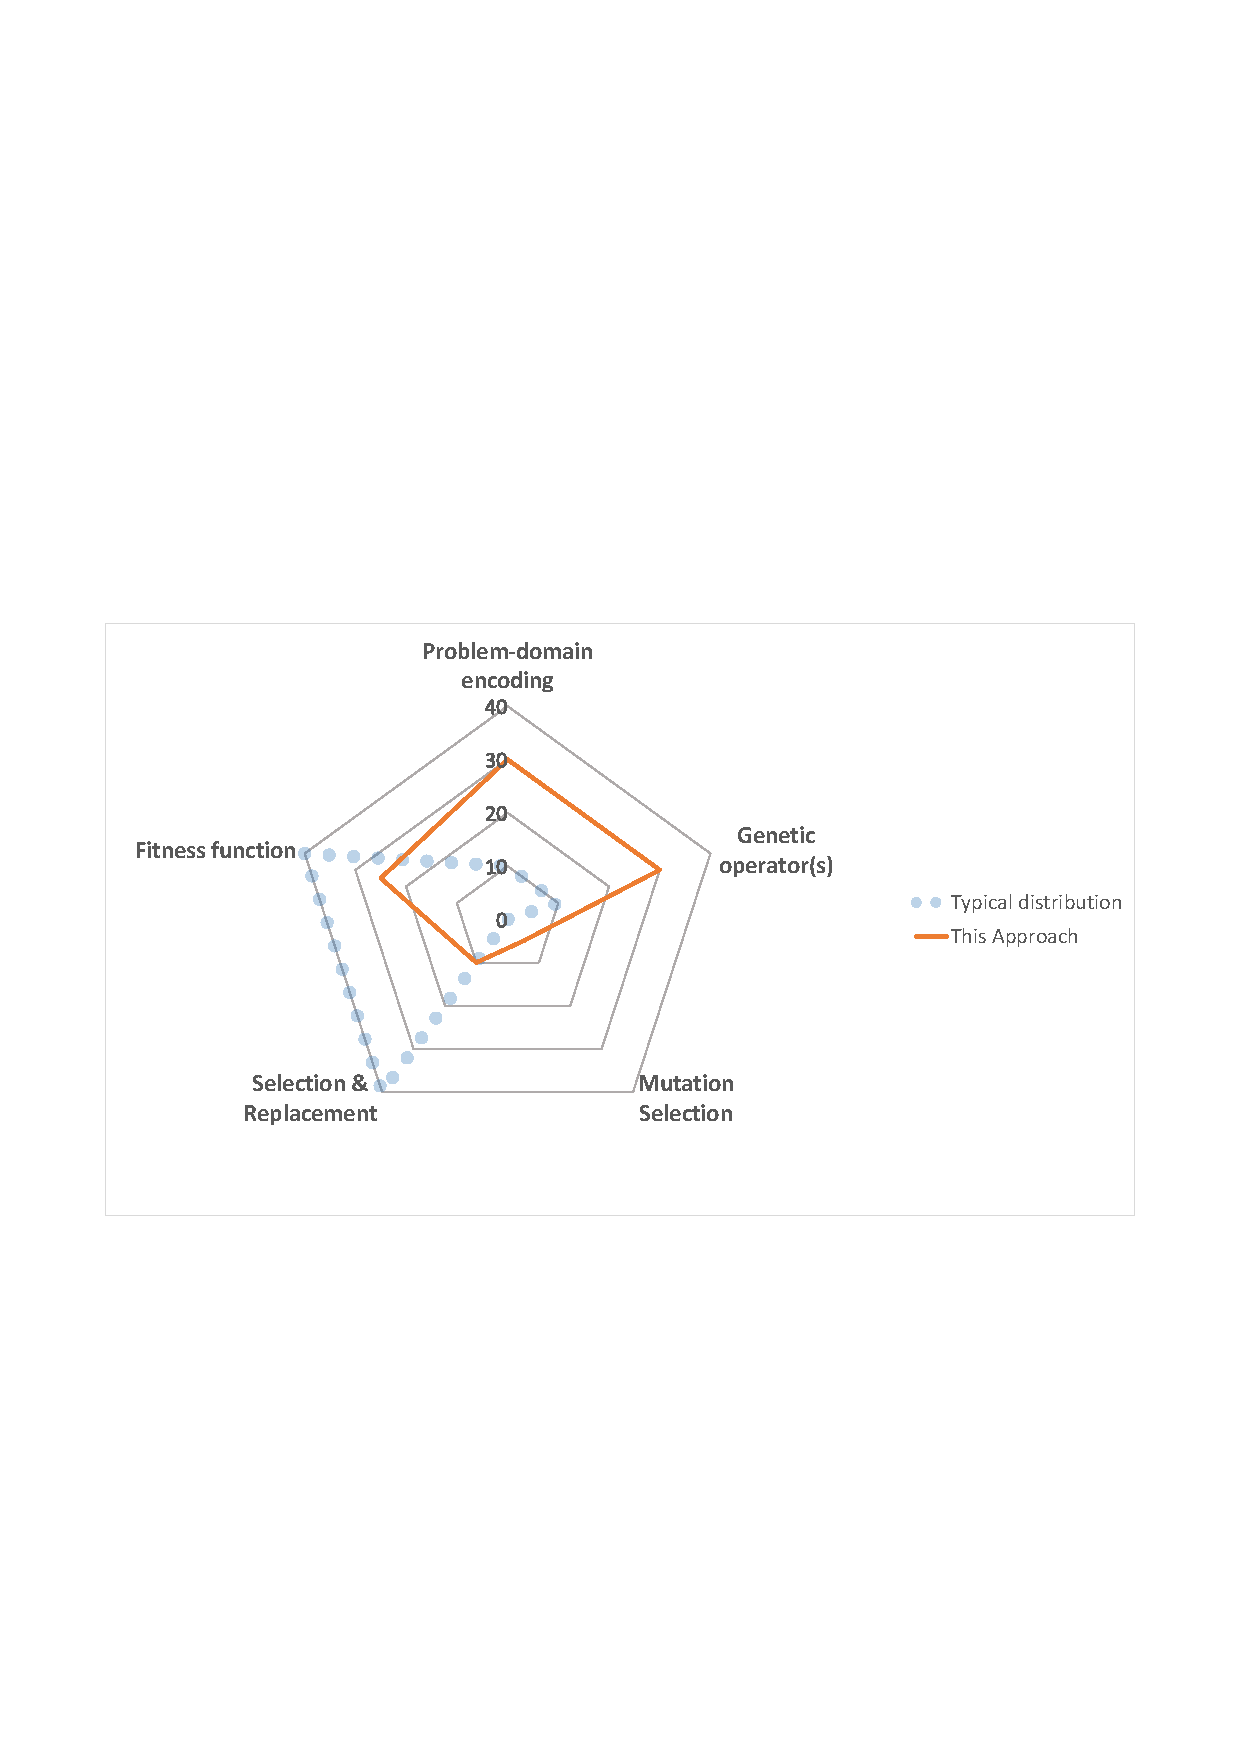
\includegraphics[scale=0.7, trim=2cm 9.3cm 2cm 10.8cm, clip=true]{Images/FocusDistribution.pdf} %scale=0.7, trim=3.5cm 9.8cm 3.5cm 11.2cm, clip=true
	\caption{Algorithm complexity distribution - approximated in \%}
	\label{figFocusDistribution}
\end{figure}

The domain of \glspl{ModelToModelTransformation} does not contain a precise and generic definition of \glspl{ModelToModelTransformation}. The existing \glspl{DomainSpecificLanguage} provide only a few constraints.  Thus, the problem of \glspl{ModelToModelTransformation} has a large scope. This resulted in a high complexity of the problem-domain specific encoding compared to typical evolutionary problems like i.e. the Traveling Salesman Problem \cite{Cickova2008}.

In the presented algorithm, the complexity is handled by multiple \glspl{GeneticOperator} which support a subset of the language capabilities. Thus, the complexity is limited. In order to avoid creating an inextensible solution, the approach is not based on an own language. The \glspl{GeneticOperator} are defined on the \gls{AbstractSyntax}. Hence, they can be extended in any required direction. Compared to other \glspl{EvolutionaryAlgorithm}, the closest description of the approach is named ``Strongly Typed Genetic Programming Algorithm" (see \cite{Montana2002}). This type is challenging, but the presented approach is also more complex as explained in sub-section \ref{subsecEvolutionaryAlgorithmFramework}.

Due to the large number of \glspl{GeneticOperator} in the form of \glspl{Mutation} with its context specific options, also the selection of those must be covered. Mutation Selection Strategies are used in the approach to handle this task. The number of options is not evenly distributed among all \glspl{Mutation}. Thus, the strategy ``Select operator first and then an option", which randomly selects the \gls{Mutation} first, outperformed the direct selection of an option. Thereby, all \glspl{Mutation} had the same probability to be chosen. In typical applications of \glspl{EvolutionaryAlgorithm} there are not that many possible \glspl{Mutation}, hence such strategies do not exist at all.

Overall the common \glspl{SelectionStrategy} and \glspl{ReplacementStrategy} were outperformed by a simple one called ``Naive approach with high selection pressure and elitism". The reason is that the naive approach evolved a broad range of \glspl{ModelToModelTransformation}, which resulted in the termination with a solution in an earlier \gls{Generation} compared to the other strategies. Nevertheless, this strategy requires more computational power per \gls{Generation} which increases the execution time. The prototype executed the \glspl{Mutation} in parallel per \gls{Generation}, which reduced this impact and rendered the naive strategy superior.

The \gls{FitnessFunction} consists of two aspects: On the one hand of the comparison method, which is a non-trivial heuristic. On the other hand of a rather simple function that aggregates the resulting differences into a fitness value. In the evaluation the heuristic performed better than a pure identity comparison, because it enabled the algorithm to detect fine grained differences between M$_b^*$ and M$_b$. Furthermore, the heuristic is fault-tolerant regarding human error. In the case the domain experts does not correctly specify the names of the \glspl{Object}, the pure identify function is unable to find any match. This results in a low fitness, even when the \gls{ModelToModelTransformation} is close to a solution. The heuristic only reduces the fitness due to the wrong identity, but is still able to provide the correct fitness for all other aspects of the \glspl{Object}.

%As defined in the goals, the created \glspl{ModelToModelTransformation} might be incomplete and hence need to be refined manually. Usually an \glspl{EvolutionaryAlgorithm} is expected to return the correct solution, which renders this approach special within this category.

%The identification of a solution can be advanced by adding additional computational power. Thereby the algorithm is able to use i.e. a larger \gls{Population} which increases the entropy resulting in a higher probability to find a solution. This dimension was not specifically targeted by the approach.